\documentclass[12pt, letterpaper]{article}
\usepackage[margin=1in]{geometry}
\usepackage[T1]{fontenc}
\usepackage{lmodern}
\usepackage{cmap}
\usepackage[utf8]{inputenc}
\usepackage{amsmath, amssymb, amsthm}
\usepackage{mathtools}
\usepackage{enumitem}
\usepackage{booktabs}
\usepackage{xcolor}
\usepackage{titlesec}
\usepackage{parskip}
\usepackage{hyperref}
\usepackage{fancyhdr}
\usepackage{tcolorbox}
\usepackage{graphicx}
\usepackage{caption}
\tcbuselibrary{skins, breakable}

\definecolor{darkblue}{RGB}{15,55,115}
\definecolor{midblue}{RGB}{30,100,180}
\definecolor{theorybg}{RGB}{245,250,255}
\definecolor{questionbg}{RGB}{255,252,240}
\definecolor{evencolor}{RGB}{60,0,100}

\hypersetup{colorlinks=true,linkcolor=darkblue,urlcolor=midblue,
  pdftitle={Kurlat --- A Course in Modern Macroeconomics --- Complete Solutions, Chapter 7}}

\setlength{\headheight}{14pt}
\pagestyle{fancy}
\fancyhf{}
\renewcommand{\headrulewidth}{0.4pt}
\fancyhead[L]{\small\textcolor{darkblue}{\textit{Kurlat --- A Course in Modern Macroeconomics}}}
\fancyhead[R]{\small\textcolor{darkblue}{\thepage}}
\fancyfoot[C]{\small\textcolor{gray}{Complete Solutions --- Chapter 7}}

\titleformat{\section}[block]
  {\large\bfseries\color{darkblue}}{}{0pt}{}
  [\vspace{2pt}\color{darkblue}\rule{\textwidth}{1.5pt}\vspace{4pt}]

\titleformat{\subsection}[block]
  {\normalsize\bfseries\color{midblue}}{}{0pt}{}
  [\vspace{1pt}\color{midblue}\rule{0.5\textwidth}{0.8pt}\vspace{3pt}]

\tcbset{
  theorybox/.style={
    enhanced,breakable,colback=theorybg,colframe=darkblue,
    fonttitle=\bfseries\small\color{darkblue},boxrule=0.5pt,arc=3pt,
    left=6pt,right=6pt,top=4pt,bottom=4pt,title={Key Theory},
  },
  questionbox/.style={
    enhanced,breakable,colback=questionbg,colframe=gray!60,
    fonttitle=\bfseries\small\color{gray!60!black},boxrule=0.4pt,arc=2pt,
    left=6pt,right=6pt,top=4pt,bottom=4pt,title={\textit{Question}},
  },
  oddbox/.style={
    enhanced,breakable,colback=white,colframe=darkblue,
    attach boxed title to top left={yshift=-2mm,xshift=6mm},
    boxed title style={colback=darkblue,colframe=darkblue,arc=2pt,
      boxrule=0pt,left=6pt,right=6pt,top=3pt,bottom=3pt},
    fonttitle=\bfseries\large\color{white},
    boxrule=0.8pt,arc=3pt,
    left=8pt,right=8pt,top=10pt,bottom=6pt,
  },
  evenbox/.style={
    enhanced,breakable,colback=white,colframe=evencolor,
    attach boxed title to top left={yshift=-2mm,xshift=6mm},
    boxed title style={colback=evencolor,colframe=evencolor,arc=2pt,
      boxrule=0pt,left=6pt,right=6pt,top=3pt,bottom=3pt},
    fonttitle=\bfseries\large\color{white},
    boxrule=0.8pt,arc=3pt,
    left=8pt,right=8pt,top=10pt,bottom=6pt,
  },
  databox/.style={
    enhanced,breakable,colback=gray!8,colframe=gray!55,
    fonttitle=\bfseries\small\color{gray!60!black},boxrule=0.4pt,arc=2pt,
    left=6pt,right=6pt,top=4pt,bottom=4pt,title={Numerical exercise --- see the companion code},
  },
  trapbox/.style={
    enhanced,breakable,colback=red!4,colframe=red!45!black,
    fonttitle=\bfseries\small\color{white},boxrule=0.4pt,arc=2pt,
    coltitle=white,
    left=6pt,right=6pt,top=4pt,bottom=4pt,title={Where this goes wrong},
  },
}

\newcommand{\pd}[2]{\dfrac{\partial #1}{\partial #2}}
\newcommand{\dd}[2]{\dfrac{d #1}{d #2}}
\newcommand{\MRS}{\mathrm{MRS}}
\newcommand{\MRT}{\mathrm{MRT}}
\newcommand{\MU}{\mathrm{MU}}
\newcommand{\Var}{\mathrm{Var}}
\newcommand{\Cov}{\mathrm{Cov}}
\newcommand{\E}{\mathrm{E}}
\newcommand{\MPK}{\mathrm{MPK}}
\newcommand{\MPL}{\mathrm{MPL}}
\newcommand{\stst}{^{\ast}}

\setlist[enumerate,1]{label=(\alph*),itemsep=6pt,parsep=2pt}
\setlist[enumerate,2]{label=(\roman*),itemsep=3pt}


\begin{document}

%======================================================================
% TITLE PAGE
%======================================================================
\begin{titlepage}
\centering
\vspace*{2.5cm}
{\Huge\bfseries\color{darkblue} A Course in Modern Macroeconomics\par}
\vspace{6pt}
{\large Pablo Kurlat (2020)\par}
\vspace{1.4cm}
{\LARGE\bfseries Complete Solutions\par}
\vspace{6pt}
{\LARGE\bfseries Chapter 7 --- Labor and Leisure\par}
\vspace{1.2cm}
{\large All seven end-of-chapter problems, 7.1--7.7 (pp.~146--150)\par}
\vspace{2cm}

\begin{tcolorbox}[theorybox,title={What is in this file},width=0.86\textwidth]
\small
Every problem carries the full question text, a step-by-step solution with no skipped
algebra, an economic reading of the result, and a verification. Numerical answers are
reproduced by the companion scripts in \texttt{Resolucao/kurlat\_ch07\_codigo/}, which
check each analytical formula against an independent computation --- a direct numerical
maximisation of the household's problem, a brute-force grid search, finite differences or a
root finder --- and abort on any mismatch.

\smallskip
Problems are grouped by \textbf{topic}, not by number, following the order of the
chapter's own sections. Blue boxes are odd-numbered problems, purple boxes even.

\smallskip
\textbf{Kurlat publishes no answer key}, so every result here is verified by other means:
executed numerical checks (marked \checkmark), first-order conditions and budget constraints
substituted back, and limiting cases.

\smallskip
Companion to \texttt{kurlat\_solutions\_ch1-4.tex}, \texttt{...\_ch05.tex},
\texttt{...\_ch06.tex} and \texttt{...\_ch09.tex}. Chapter 8 is outside the course syllabus.
\end{tcolorbox}

\vfill
{\small MPE Insper --- Macroeconomia I --- 2026, 3\textordmasculine{} trimestre\par}
\end{titlepage}

\tableofcontents
\newpage

%======================================================================
\section{Chapter 7 \quad Labor and Leisure}
%======================================================================

\begin{tcolorbox}[theorybox,title={Chapter 7 Overview}]
The chapter turns the choice of hours into a two-good consumption problem: the household
sells part of its one unit of time to buy goods.

\smallskip
\textbf{The problem.} Maximise $u(c)+v(l)$ subject to $c\le w(1-l)(1-\tau)+T$, with
$L=1-l$ hours of market work. The first-order condition (7.2.3), with the after-tax wage in
place of $w$, is
\[
\frac{v'(l)}{u'(c)}=w(1-\tau)
\]
--- the marginal rate of substitution between leisure and consumption equals the after-tax
price of time.

\smallskip
\textbf{Income and substitution.} A higher wage makes leisure dearer (substitution: work
more) and makes the household richer (income: work less). Which one wins depends on
preferences: in the explicit example (7.2.4) hours rise with $w$ if $\sigma<1$, fall if
$\sigma>1$, and are flat with $\sigma=1$. The evidence (\S7.3) says the two effects almost
cancel, with the income effect slightly ahead.

\smallskip
\textbf{Taxes and transfers.} A transfer $T$ is a pure income effect (more leisure). A tax
$\tau$ is like a lower wage --- both effects. A tax whose revenue comes back as a transfer
keeps the substitution effect and cancels the income effect, which is why it reduces hours
unambiguously. That is Prescott's argument for the US--Europe gap (Problem 7.5).

\smallskip
\textbf{Equilibrium.} Competitive: labour demand $w=F_L(K,L)$ meets labour supply.
Search (Diamond--Mortensen--Pissarides): firms post vacancies at cost $\chi$ until
\[
\chi=q(V,U)(1-\mu)(y-b), \tag{7.5.1}
\]
and after-hiring unemployment is $U'=U-m(V,U)$ (7.5.2). Anything that makes firms post more
vacancies with $U$ given lowers $U'$: a Beveridge curve.
\end{tcolorbox}

\newpage
%---- Topic: The Consumption-Leisure Choice ----
\subsection{The Consumption--Leisure Choice}

%------- 7.1 -------
% Topic: The Consumption-Leisure Choice
% Keywords: quasi-linear utility, no income effect, labour supply, cross-country evidence
\begin{tcolorbox}[oddbox,title={Problem 7.1 \quad Labor Supply}]
\begin{tcolorbox}[questionbox]
Suppose household preferences are given by:
\[u(c,l)=c+\theta\log(l)\]
where $c$ is consumption, $l$ is leisure and $\theta$ is a parameter. Households have a total
of one unit of time and can supply labor in a competitive labor market at a wage $w$.\\[3pt]
(a) Find an expression for the fraction of their time that households spend in market work.\\
(b) If this was the right model and one looked at households in different countries, how
would hours of work correlate with wage levels? How does this compare to the empirical
evidence?
\end{tcolorbox}

\textbf{Solution:}

\begin{enumerate}
\item The household solves $\max_{c,l}\;c+\theta\log l$ subject to $c\le w(1-l)$. The
Lagrangian is
\[
\mathcal{L}(c,l,\lambda)=c+\theta\log l-\lambda\,[\,c-w(1-l)\,].
\]
First-order conditions:
\[
\pd{\mathcal L}{c}=1-\lambda=0\;\Rightarrow\;\lambda=1,
\qquad
\pd{\mathcal L}{l}=\frac{\theta}{l}-\lambda w=0\;\Rightarrow\;\frac{\theta}{l}=w .
\]
This is (7.2.3) with $u'(c)=1$ and $v'(l)=\theta/l$. Solving,
\[
l=\frac{\theta}{w}
\qquad\Longrightarrow\qquad
\boxed{\,1-l=1-\frac{\theta}{w}\,}\qquad\text{if } w>\theta .
\]
Leisure cannot exceed the time endowment. If $w\le\theta$ the interior solution would give
$l\ge1$, so the household sits at the corner $l=1$ and works \textbf{zero} hours. Combining,
$1-l=\max\{0,\,1-\theta/w\}$, and consumption is $c=w(1-l)=w-\theta$ when $w>\theta$.

\emph{Reading.} Utility is linear in $c$, so the marginal utility of consumption is
constant at one: extra income never makes consumption less valuable, and there is
\textbf{no income effect} on leisure. The only force left is substitution. Leisure is set
where its marginal utility $\theta/l$ equals its price $w$, whatever the household's wealth.

\item Differentiate hours with respect to the wage (interior case):
\[
\dd{(1-l)}{w}=\frac{\theta}{w^{2}}>0 ,
\qquad
\lim_{w\to\infty}(1-l)=1 .
\]
So hours are \textbf{strictly increasing} in the wage: countries with higher wages would work
more, and the richest would devote almost all their time to market work. With $\theta=0.4$:

\begin{center}
\begin{tabular}{@{}cccc@{}}
\toprule
$w$ & $l=\theta/w$ & hours $1-l$ & $l$ (numerical maximisation)\\
\midrule
0.50 & 0.8000 & 0.2000 & 0.8000\\
1.00 & 0.4000 & 0.6000 & 0.4000\\
2.00 & 0.2000 & 0.8000 & 0.2000\\
5.00 & 0.0800 & 0.9200 & 0.0800\\
20.00 & 0.0200 & 0.9800 & 0.0200\\
\bottomrule
\end{tabular}
\end{center}

\textbf{Evidence.} It goes the other way. Across countries (Bick et al.\ 2018, Figure
7.3.2) hours worked are \emph{negatively} correlated with GDP per capita, although weakly;
over time in the US (Ramey and Francis 2009, Figure 7.3.1), wages rose about ninefold in a
century while leisure rose slightly. Both say that income and substitution effects nearly
cancel, with the income effect a little stronger. The quasi-linear model has the
\textbf{wrong sign}, and it gets it wrong precisely because it has switched off the income
effect.

\emph{Contrast.} With $u=\log c+\alpha\log l$ the two effects cancel exactly and hours are
$1/(1+\alpha)$ at every wage (for $\alpha=1.54$, $0.3937$); with (7.2.4) and $\sigma>1$ hours
fall with the wage, which is the sign in the data (Figure~\ref{fig:oferta71}).
\end{enumerate}

\begin{center}
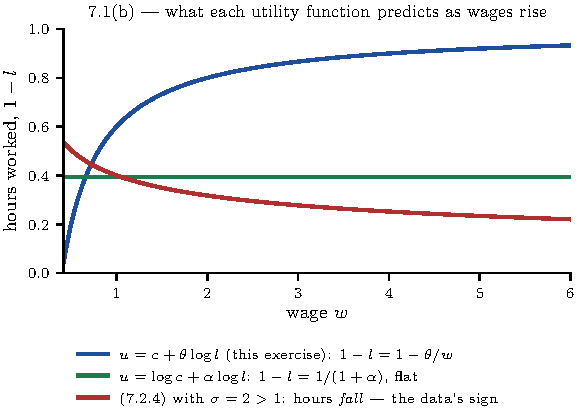
\includegraphics[width=0.72\linewidth]{fig/fig_k7_1_oferta.pdf}\\[3pt]
\captionof{figure}{Problem 7.1(b). Hours against the wage under three utility functions
($\theta=0.4$). Only curvature in $u(c)$ strong enough for the income effect to win
($\sigma>1$) matches the negative cross-country correlation.}
\label{fig:oferta71}
\end{center}

\textbf{Verification.} Direct numerical maximisation of $c+\theta\log l$ over the budget line
reproduces $l=\theta/w$ at every wage in the table, and confirms that the log--log case gives
$l=\alpha/(1+\alpha)$ at $w=0.5,\,2,\,20$. \checkmark
\end{tcolorbox}

%------- 7.2 -------
% Topic: The Consumption-Leisure Choice
% Keywords: lump-sum tax, conscription, in-kind tax, equivalence
\begin{tcolorbox}[evenbox,title={Problem 7.2 \quad Military Service}]
\begin{tcolorbox}[questionbox]
An economy is populated by a representative household, whose preferences are described by:
\[u(c)+v(l)\]
where $c$ is consumption and $l$ is leisure. The household has 1 unit of time so its budget
is:
\[c=w(1-l)-\tau\]
where $w$ is the wage rate and $\tau$ is a tax that the government collects. Notice that
$\tau$ is a lump-sum tax, not an income tax: the household must pay the same amount
regardless of how much income it earns.\\[3pt]
(a) Set up the Lagrangian for the household's optimization program and find first-order
conditions.\\
(b) Use the budget constraint to replace $c$ in the first-order condition to obtain a single
equation that relates the household's choice of $l$ to $w$ and $\tau$.\\
(c) Suppose that the government uses all the tax revenue to hire soldiers for the army,
paying them the prevailing wage rate. How many units of soldiers' time can the government
afford? Denote this number by $m$.\\
(d) Now suppose that instead of taxing citizens to hire soldiers, the government imposes
compulsory military service: the representative household has to dedicate $m$ units of time
to serving in the army, unpaid. The rest of their time they can use as they please, and they
pay no taxes. Set up the household's optimization program under this policy.\\
(e) Show that the representative household's level of consumption, leisure, army labor and
non-army labor are the same under both policies. Explain.
\end{tcolorbox}

\textbf{Solution:}

\begin{enumerate}
\item The Lagrangian is
\[
\mathcal L(c,l,\lambda)=u(c)+v(l)-\lambda\,[\,c-w(1-l)+\tau\,].
\]
First-order conditions:
\[
\pd{\mathcal L}{c}=u'(c)-\lambda=0,
\qquad
\pd{\mathcal L}{l}=v'(l)-\lambda w=0,
\qquad
\pd{\mathcal L}{\lambda}=0\;\Leftrightarrow\;c=w(1-l)-\tau .
\]
Eliminating $\lambda=u'(c)$ from the second:
\[
\boxed{\;\frac{v'(l)}{u'(c)}=w\;}
\]
--- exactly (7.2.3). The lump-sum tax does not appear: it does not change the price of time.

\item Substitute $c=w(1-l)-\tau$:
\[
\boxed{\;v'(l)=w\,u'\!\big(w(1-l)-\tau\big)\;}
\]
One equation in one unknown $l$, given $w$ and $\tau$. Since $u'$ is decreasing, a higher
$\tau$ lowers $c$ at any $l$ and raises the right-hand side; with $v'$ decreasing, the
equality is restored at a \emph{lower} $l$. A lump-sum tax is a pure (negative) income effect
and makes the household work more.

\item The revenue is $\tau$ and one unit of soldiers' time costs $w$, so
\[
\boxed{\;m=\frac{\tau}{w}\;}.
\]

\item The household loses $m$ units of time and pays no tax. It has $1-m$ units left to
split between leisure and paid work, so paid work is $1-m-l$ and
\[
\max_{c,l}\;u(c)+v(l)
\quad\text{s.t.}\quad c=w(1-m-l),\qquad 0\le l\le1-m .
\]
Lagrangian $\mathcal L=u(c)+v(l)-\lambda[c-w(1-m-l)]$, with first-order conditions
$u'(c)=\lambda$ and $v'(l)=\lambda w$, so again $v'(l)/u'(c)=w$, and substituting the
constraint, $v'(l)=w\,u'\big(w(1-m-l)\big)$.

\item Expand the conscription budget and use $m=\tau/w$ from (c):
\[
c=w(1-m-l)=w(1-l)-wm=w(1-l)-w\cdot\frac{\tau}{w}=w(1-l)-\tau .
\]
This is \emph{the same budget line} as under the tax, and the objective is the same, so the
optimal $(c,l)$ are identical --- the equations in (b) and (d) are literally the same
equation. Then:
\begin{itemize}
\item \textbf{Army labour} is $m=\tau/w$ in both cases: hired with the tax revenue in one,
drafted in the other.
\item \textbf{Non-army labour} is $1-l-m$ in both cases: under the tax the household works
$1-l$ in total, of which $m$ is sold to the army; under the draft it serves $m$ and works
$1-m-l$ in the market.
\end{itemize}

\emph{Explanation.} Both policies are \textbf{lump-sum}: neither depends on anything the
household chooses at the margin, so neither changes the price of time, which is $w$ in both.
Both take the same resources, $wm=\tau$ units of goods (or $m$ units of time valued at $w$).
The draft is a lump-sum tax collected in kind --- in time instead of goods. With a
competitive labour market, paying $\tau$ and working $m$ extra hours at wage $w$ are the
same thing.
\end{enumerate}

\begin{tcolorbox}[databox]
With $w=2$, $\tau=0.3$, $u(c)=\frac{c^{1-\sigma}-1}{1-\sigma}$ with $\sigma=2$ and
$v(l)=3\,\frac{l^{1-\eta}-1}{1-\eta}$ with $\eta=1.5$, so $m=0.3/2=0.150$:

\begin{center}
\begin{tabular}{@{}lcccc@{}}
\toprule
policy & leisure $l$ & consumption $c$ & army $m$ & non-army $1-l-m$\\
\midrule
lump-sum tax & 0.579017 & 0.541967 & 0.150 & 0.270983\\
conscription & 0.579017 & 0.541967 & 0.150 & 0.270983\\
\bottomrule
\end{tabular}
\end{center}
Check of the budget: $c=2(1-0.579017)-0.3=0.841966-0.3=0.541966$. Check of the first-order
condition: $v'(l)/u'(c)=3l^{-1.5}/c^{-2}=3c^{2}/l^{1.5}=3(0.293728)/0.440596=0.881184/0.440596
=2.000=w$. \checkmark
\end{tcolorbox}

\begin{tcolorbox}[trapbox]
The equivalence is a property of the \emph{representative} household. With heterogeneous
workers a draft of $m$ hours per person costs a surgeon far more (in foregone $w$) than it
costs a low-wage worker, while a tax-financed volunteer army hires whoever has the lowest
opportunity cost. The aggregate resource cost is then \emph{not} the same, and the draft is
the more expensive one. The exercise shows that the draft is a tax, not that it is a good one.
\end{tcolorbox}
\end{tcolorbox}

\newpage
%---- Topic: Taxes, Transfers and Labour Supply ----
\subsection{Taxes, Transfers and Labour Supply}

%------- 7.3 -------
% Topic: Taxes, Transfers and Labour Supply
% Keywords: consumption tax, income tax, wedge, tax equivalence, revenue
\begin{tcolorbox}[oddbox,title={Problem 7.3 \quad Consumption Taxes and Labor Supply}]
\begin{tcolorbox}[questionbox]
Suppose a household solves the following problem:
\[
\max_{c,l}\;u(c)+v(l)\quad\text{s.t.}\quad(1+\tau_c)c\le w(1-\tau)(1-l)
\]
where $c$ is consumption, $l$ is leisure and $\tau$ is an income tax. $\tau_c$ is a
consumption tax, so that if the household wishes to consume $c$ it must pay $(1+\tau_c)c$.\\[3pt]
(a) Draw the household's budget constraint. What is the slope?\\
(b) Find the first-order conditions for the household's consumption-leisure decision. How do
the effects of $\tau$ and $\tau_c$ relate to each other? Explain.\\
(c) If the household chooses $c^*$ and $l^*$, how much tax revenue does the government
collect?\\
(d) Suppose the government had originally set $\tau_c=0$ and $\tau>0$ and now wants to enact
a tax reform that uses consumption taxes instead of income taxes. What would be the level of
$\tau_c$ that leaves the decisions of the household unchanged?\\
(e) How much revenue does the government collect under the new system? How does it compare
to the old system? Explain.
\end{tcolorbox}

\textbf{Solution:}

\begin{enumerate}
\item Solving the constraint for $c$ (it binds, since $u'>0$):
\[
c=\frac{w(1-\tau)}{1+\tau_c}\,(1-l).
\]
In the $(l,c)$ plane this is a straight line through $(1,0)$ --- all time as leisure, no
consumption --- with vertical intercept $c=\frac{w(1-\tau)}{1+\tau_c}$ at $l=0$. Its slope is
\[
\boxed{\;\dd{c}{l}=-\frac{w(1-\tau)}{1+\tau_c}\;}.
\]
Either tax rotates the line clockwise about $(1,0)$, making it flatter:

\begin{center}
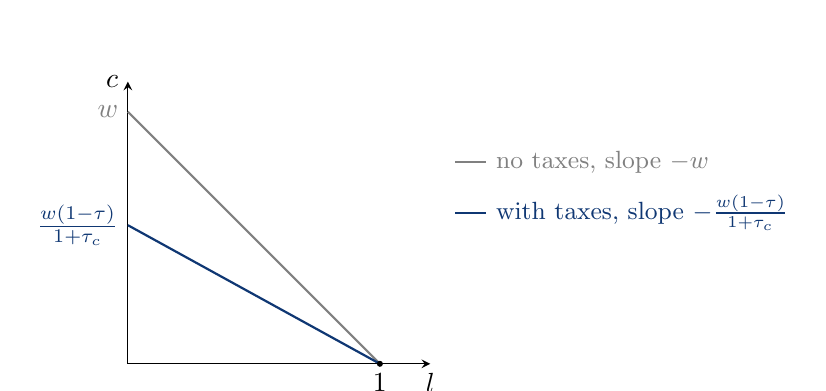
\begin{tikzpicture}[scale=3.2,>=stealth]
\draw[->] (0,0) -- (1.2,0) node[below] {$l$};
\draw[->] (0,0) -- (0,1.12) node[left] {$c$};
\draw[thick,gray] (0,1) -- (1,0);
\draw[thick,darkblue] (0,0.55) -- (1,0);
\node[left,gray] at (0,1) {$w$};
\node[left,darkblue] at (0,0.55) {$\frac{w(1-\tau)}{1+\tau_c}$};
\node[below] at (1,0) {$1$};
\draw[thick,gray] (1.3,0.8) -- (1.42,0.8) node[right] {\small no taxes, slope $-w$};
\draw[thick,darkblue] (1.3,0.6) -- (1.42,0.6) node[right] {\small with taxes, slope $-\frac{w(1-\tau)}{1+\tau_c}$};
\fill (1,0) circle (0.012);
\end{tikzpicture}
\end{center}

\item Lagrangian:
\[
\mathcal L=u(c)+v(l)-\lambda\,[(1+\tau_c)c-w(1-\tau)(1-l)].
\]
First-order conditions:
\[
\pd{\mathcal L}{c}=u'(c)-\lambda(1+\tau_c)=0,\qquad
\pd{\mathcal L}{l}=v'(l)-\lambda w(1-\tau)=0.
\]
Dividing the second by the first:
\[
\boxed{\;\frac{v'(l)}{u'(c)}=\frac{w(1-\tau)}{1+\tau_c}\;}.
\]
The two taxes enter \textbf{only through the single wedge} $\frac{1-\tau}{1+\tau_c}$, both in
the first-order condition and in the budget constraint. So they are perfect substitutes: any
two pairs $(\tau,\tau_c)$ with the same $\frac{1-\tau}{1+\tau_c}$ produce the same choices.
Raising $1+\tau_c$ by some factor has exactly the effect of cutting $1-\tau$ by that factor.

\emph{Explanation.} The household's only decision is how much time to convert into goods. An
income tax cuts the goods received per hour on the way in; a consumption tax cuts them on the
way out. Either way the household gets $\frac{w(1-\tau)}{1+\tau_c}$ units of consumption per
hour given up, and that real after-tax wage is all that matters to it.

\item Revenue is income-tax revenue plus consumption-tax revenue:
\[
R=\tau w(1-l^*)+\tau_c c^* .
\]
Replacing $c^*=\frac{w(1-\tau)}{1+\tau_c}(1-l^*)$:
\[
R=w(1-l^*)\left[\tau+\frac{\tau_c(1-\tau)}{1+\tau_c}\right]
=w(1-l^*)\,\frac{\tau+\tau\tau_c+\tau_c-\tau_c\tau}{1+\tau_c}
=\boxed{\;w(1-l^*)\,\frac{\tau+\tau_c}{1+\tau_c}\;}.
\]
Equivalently $R=w(1-l^*)-c^*$, since
$w(1-l^*)-c^*=w(1-l^*)\big[1-\frac{1-\tau}{1+\tau_c}\big]
=w(1-l^*)\frac{\tau+\tau_c}{1+\tau_c}$: revenue is whatever of the household's output it
does not consume.

\item Decisions are unchanged if the wedge is unchanged:
\[
\frac{1-0}{1+\tau_c}=\frac{1-\tau}{1+0}
\;\Longrightarrow\;
1+\tau_c=\frac{1}{1-\tau}
\;\Longrightarrow\;
\boxed{\;\tau_c=\frac{\tau}{1-\tau}\;}.
\]
With the same wedge, the budget line of (a) and the first-order condition of (b) are the
same, so the household picks the same $(c^*,l^*)$. For $\tau=0.3$,
$\tau_c=0.3/0.7=0.428571$: a 30\% income tax is a 42.9\% consumption tax (the consumption
tax is quoted on a tax-exclusive base, the income tax on a tax-inclusive one).

\item Using (c) with $\tau=0$ and $\tau_c=\frac{\tau}{1-\tau}$, so that
$1+\tau_c=\frac{1}{1-\tau}$:
\[
R^{\text{new}}=w(1-l^*)\frac{\tau_c}{1+\tau_c}
=w(1-l^*)\,\frac{\tau/(1-\tau)}{1/(1-\tau)}
=\tau\,w(1-l^*)=R^{\text{old}} .
\]
\textbf{Exactly the same revenue.} The reason is $R=w(1-l^*)-c^*$: output and consumption are
both unchanged, so what the government collects must be unchanged too. In this static model
the household consumes all of its after-tax earnings, so the consumption-tax base \emph{is}
labour income; taxing it when it is spent is the same as taxing it when it is earned.
\end{enumerate}

\begin{tcolorbox}[databox]
With $w=2$, $\tau=0.3$ and the preferences of Problem 7.2 ($\sigma=2$, $\eta=1.5$): the
income tax alone gives $l^*=0.64770396$; the consumption tax $\tau_c=0.428571$ alone gives
$l^*=0.64770396$. Consumption is $c^*=1.4\times0.35229604=0.49321446$ in both; revenue is
$\tau w(1-l^*)=0.6\times0.35229604=0.21137763$ in both, and equals
$w(1-l^*)-c^*=0.70459208-0.49321446$. Every pair on the iso-wedge line
$\tau=1-(1-0.3)(1+\tau_c)$ agrees:

\begin{center}
\begin{tabular}{@{}cccc@{}}
\toprule
$\tau$ & $\tau_c$ & $l^*$ & revenue\\
\midrule
0.3000 & 0.0000 & 0.647704 & 0.211378\\
0.1950 & 0.1500 & 0.647704 & 0.211378\\
0.0900 & 0.3000 & 0.647704 & 0.211378\\
0.0000 & 0.4286 & 0.647704 & 0.211378\\
\bottomrule
\end{tabular}
\end{center}
\end{tcolorbox}

\begin{tcolorbox}[trapbox]
The equivalence rests on the household having \emph{no other resources}. With initial wealth,
savings or transfers, a consumption tax also taxes consumption financed out of wealth ---
a lump-sum element --- and the two taxes stop being equivalent in both allocation and
revenue. Here $c^*$ is financed entirely by current labour income, which is what makes the
two bases coincide.
\end{tcolorbox}
\end{tcolorbox}

%------- 7.4 -------
% Topic: Taxes, Transfers and Labour Supply
% Keywords: transfers, means testing, implicit tax, non-participation, minimum wage
\begin{tcolorbox}[evenbox,title={Problem 7.4 \quad Puerto Rico}]
\begin{tcolorbox}[questionbox]
Read the following article:
\url{https://www.economist.com/united-states/2006/05/25/trouble-on-welfare-island}. Is what
was going on in Puerto Rico consistent with the theories discussed in this chapter? Discuss.
\end{tcolorbox}

\textbf{Solution:}

\emph{A note on the source.} The article is behind a paywall and could not be retrieved when
these solutions were written, so the answer below does not quote it. It rests on the
chapter's model and on the broad, well-documented facts the article's title points to:
Puerto Rico's labour-force participation was far below the mainland's (well under half of
the adult population, against roughly two-thirds on the mainland), while residents were
covered by federal transfer programmes and the federal minimum wage, both set with mainland
incomes in mind.

\textbf{The short answer: yes, it is what the chapter predicts.} Three mechanisms of the
chapter are at work.

\begin{enumerate}
\item \textbf{Transfers have a pure income effect.} In \S7.2 a transfer $T$ shifts the budget
line up without changing its slope; the household buys more of every normal good, leisure
included (Figure 7.2.4). What matters is the size of $T$ \emph{relative to the wage}. With
$u=\log c+\alpha\log l$ and budget $c=w(1-\tau)(1-l)+T$, Problem 7.5(b) gives
\[
l=\frac{\alpha\,[w(1-\tau)+T]}{(1+\alpha)\,w(1-\tau)} ,
\]
and the household stops working altogether ($l\ge1$) when
\[
\alpha\,[w(1-\tau)+T]\ge(1+\alpha)\,w(1-\tau)
\;\Longleftrightarrow\;
\alpha T\ge w(1-\tau)
\;\Longleftrightarrow\;
\boxed{\;T\ge\frac{w(1-\tau)}{\alpha}\;}.
\]
Benefits designed for mainland wage levels, paid in an economy where wages are much lower,
make $T/w$ large --- exactly the region where the model predicts non-participation.

\item \textbf{Means-testing is an implicit tax.} Footnote 3 of the chapter makes the point: a
benefit that is withdrawn as earnings rise is a tax on earnings at the withdrawal rate. A
benefit $B$ phased out at rate $s$ gives the budget
\[
c=\max\big\{\,B+(1-s)\,w(1-l),\;w(1-l)\,\big\},
\]
with a kink at earnings $w(1-l)=B/s$ where the benefit is exhausted. On the benefit segment
it is the $(\tau,T)=(s,B)$ budget: the income effect of $B$ and the substitution effect of the
tax $s$ \emph{both} push toward leisure. The upper envelope of two lines is a \textbf{non-convex}
budget set, so the response of hours to the benefit can be discontinuous: a household either
works past the phase-out range or drops to low hours on the benefit segment.

\item \textbf{A wage floor above the competitive wage.} In the competitive labour market of
\S7.5 firms hire until $w=F_L(K,L)$. If the federal minimum wage $\bar w$ is above the wage at
which that demand curve meets labour supply --- plausible where productivity is well below the
mainland's --- firms hire only $L^d$ with $F_L(K,L^d)=\bar w$, less than households want to
supply. The shortfall is non-employment the household did not choose, and some of the labour
that remains moves into informal work, which official hours do not record.
\end{enumerate}

\textbf{A worked illustration of mechanism 2.} Take $\alpha=1.54$, $w=1$ and a phase-out rate
$s=0.5$.

\emph{Benefit segment.} By the formula above with $\tau=s$, $T=B$:
$l_1=\frac{\alpha(w(1-s)+B)}{(1+\alpha)w(1-s)}$, capped at 1. Zero hours when
$B\ge B^*=\frac{w(1-s)}{\alpha}=\frac{0.5}{1.54}=0.324675$.

\emph{No-benefit segment} ($c=w(1-l)$, $T=0$): the interior optimum is
$l_2=\frac{\alpha}{1+\alpha}=0.606299$, valid only if its earnings $0.393701$ reach the kink
$B/s$; otherwise the best point on this segment is the kink itself, $1-l=B/s$.

The household picks whichever candidate gives higher utility $\log c+\alpha\log l$:

\begin{center}
\small
\begin{tabular}{@{}c|ccc|ccc|c@{}}
\toprule
 & \multicolumn{3}{c|}{benefit segment} & \multicolumn{3}{c|}{no-benefit segment} & \\
$B$ & $l_1$ & $c$ & utility & $l_2$ & $c$ & utility & hours $1-l$\\
\midrule
0.00 & --- & --- & --- & 0.606299 & 0.393701 & $-1.702752$ & \textbf{0.393701}\\
0.15 & 0.788189 & 0.255906 & $-1.729494$ & 0.606299 & 0.393701 & $\mathbf{-1.702752}$ & \textbf{0.393701}\\
0.25 & 0.909449 & 0.295276 & $\mathbf{-1.366018}$ & 0.500000 & 0.500000 & $-1.760594$ & \textbf{0.090551}\\
0.35 & 1.000000 & 0.350000 & $\mathbf{-1.049822}$ & 0.300000 & 0.700000 & $-2.210793$ & \textbf{0}\\
\bottomrule
\end{tabular}
\end{center}

Step by step for $B=0.25$: $l_1=\frac{1.54(0.5+0.25)}{2.54\times0.5}=\frac{1.155}{1.27}
=0.909449$; earnings $0.090551<B/s=0.5$, so it is on the benefit segment; $c=0.25+0.5\times
0.090551=0.295276$; utility $\log0.295276+1.54\log0.909449=-1.219846-0.146171=-1.366018$.
The no-benefit interior would need earnings $0.393701\ge0.5$, which fails, so that segment's
best point is the kink $l=0.5$, $c=0.5$, utility $2.54\log0.5=-1.760594$. The benefit
segment wins.

\emph{Reading.} A benefit of $0.15$ changes nothing: the household earns past the phase-out
range and ignores the programme. Raising it to $0.25$ flips the household onto the benefit
segment and cuts hours by $1-0.090551/0.393701=77\%$; at $0.35>B^*$ it leaves the labour force.
Modest differences in benefits relative to wages can produce very large differences in
participation --- which is the Puerto Rican pattern.

\begin{tcolorbox}[databox]
\texttt{problema\_7\_4} solves the kinked problem by a brute-force search over two million
grid points for $l\in(0,1]$ and matches the segment-by-segment solution above at every $B$ to
within $10^{-5}$; it asserts $B^*=0.324675$, zero hours for $B=0.35$, and that hours never
rise with $B$. \checkmark
\end{tcolorbox}

\begin{tcolorbox}[trapbox]
``Consistent with'' is not ``proven by''. Low participation is also what one would see if
labour \emph{demand} were weak for reasons outside the chapter (low productivity, loss of
investment incentives), and the migration of workers to the mainland selects who stays.
Measured hours also miss informal work. And the magnitudes depend on the labour-supply
elasticity, which Problem 7.5(l) shows is easy to overstate. The chapter explains the
direction of the Puerto Rican facts; separating the three mechanisms requires evidence the
model alone does not provide.
\end{tcolorbox}
\end{tcolorbox}

%------- 7.5 -------
% Topic: Taxes, Transfers and Labour Supply
% Keywords: Prescott, US vs Europe, balanced budget, consumption-equivalent welfare, Frisch elasticity
\begin{tcolorbox}[oddbox,title={Problem 7.5 \quad Prescott's Calculation}]
\begin{tcolorbox}[questionbox]
Suppose preferences for consumption and leisure are:
\[u(c,l)=\log(c)+\alpha\log(l)\]
and households solve:
\[\max_{c,l}u(c,l)\quad\text{s.t.}\quad c=w(1-\tau)(1-l)+T\]
(a) Find first-order conditions for the consumption-leisure decision.\\
(b) Use the budget constraint to solve for leisure $l$. You should get an explicit expression
for $l$ as a function of $w$, $\tau$, $T$ and $\alpha$.\\
(c) Suppose $T=0$. How does $l$ respond to the tax rate $\tau$? What does this mean?\\[3pt]
Now suppose that in both Europe and the US we have $\alpha=1.54$, $w=1$, but in the US we
have $\tau=0.34$, $T=0.102$, while in Europe we have $\tau=0.53$, $T=0.124$.\\[3pt]
(d) Compute the amount of leisure chosen in the US and Europe. If we interpret 1 as your
entire adult lifetime, what fraction of their adult lives do people in Europe and the US
work? Comment on the respective role of taxes and transfers in this analysis using your
answers to parts (b) and (c).\\
(e) The values for $\tau$ and $T$ above are not arbitrary. If you did the calculations
correctly, you should find that both governments have balanced budgets (up to rounding
error), i.e.\ they redistribute all the tax revenue back as transfers. Check that this is the
case.\\
(f) Assuming the production function is $Y=L=1-l$, how much lower is GDP per capita in Europe
compared to the US?\\
(g) Compute the relative welfare of Europe by solving for $\lambda$ in the following equation:
\[u(c_{\text{Europe}},l_{\text{Europe}})=u(\lambda c_{\text{US}},l_{\text{US}})\]
Interpret the number $\lambda$ that you find.\\
(h) How do the answers to questions (f) and (g) compare? Why?\\
(i) Suppose a European policymaker sees Prescott's calculation and concludes that Europe could
increase its welfare by a factor of $\frac{1}{\lambda}$ by reducing its tax rate and level of
transfers to US levels. Do you think they are right? Why? Don't answer this question
mechanically: think about what this calculation does and what it leaves out.
\end{tcolorbox}
% the statement is too long for one unbreakable nested box, so it is split
\begin{tcolorbox}[questionbox,title={\textit{Question (continued)}}]
In any calculation of this sort, an important parameter is the elasticity of labor supply.
One definition of elasticity that is often looked at by labor economists is known as the
``Frisch'' elasticity. It is based on the answer to the following question: ``suppose we
increased wages but adjusted the household's income so that consumption remained constant:
how would labor supply change?'' Let's calculate the Frisch elasticity in Prescott's model.\\[3pt]
(j) Use your answer to part (a) to find an expression for labor supply $(1-l)$ in terms of
$w(1-\tau)$, $c$ and $\alpha$. Notice that now we are holding consumption constant, so the
idea is that we don't replace $c$ from the budget constraint like we did in part (b).\\
(k) Use your answer to part (j) to find an expression for
$\frac{\partial(1-l)}{\partial w(1-\tau)}\frac{w(1-\tau)}{1-l}$, i.e.\ the elasticity of labor
supply with respect to after-tax wages, holding consumption constant.\\
(l) Plug in the values of $\alpha$, $\tau$, $w$, $c$ and $l$ that you found for the US case
into the expression for elasticity. What number do you get? Empirical estimates of this
elasticity are usually in the range of 0.4 to 1. How does that compare to the elasticity
implied by Prescott's model? Why does that matter for our conclusions about tax policy?
\end{tcolorbox}

\textbf{Solution:}

\begin{enumerate}
\item Lagrangian $\mathcal L=\log c+\alpha\log l-\lambda[c-w(1-\tau)(1-l)-T]$. First-order
conditions:
\[
\frac1c=\lambda,\qquad \frac{\alpha}{l}=\lambda\,w(1-\tau)
\;\Longrightarrow\;
\frac{\alpha/l}{1/c}=w(1-\tau)
\;\Longrightarrow\;
\boxed{\;\alpha c=w(1-\tau)\,l\;}.
\]

\item Substitute $c=w(1-\tau)(1-l)+T$ into $\alpha c=w(1-\tau)l$:
\[
\alpha w(1-\tau)-\alpha w(1-\tau)\,l+\alpha T=w(1-\tau)\,l
\;\Longrightarrow\;
\alpha\,[w(1-\tau)+T]=(1+\alpha)\,w(1-\tau)\,l ,
\]
\[
\boxed{\;l=\frac{\alpha\,[w(1-\tau)+T]}{(1+\alpha)\,w(1-\tau)}
=\frac{\alpha}{1+\alpha}\left[1+\frac{T}{w(1-\tau)}\right]\;}.
\]

\item With $T=0$: $l=\frac{\alpha}{1+\alpha}$, which \textbf{does not depend on $\tau$} (nor
on $w$). For $\alpha=1.54$, $l=0.606299$ at every tax rate. A tax is a cut in the price of
time: the substitution effect pushes toward leisure, the income effect (the household is
poorer) pushes toward work, and with log utility the two cancel exactly. An income tax whose
revenue is thrown away does not change hours.

\item US:
\[
l_{US}=\frac{1.54\,(0.66+0.102)}{2.54\times0.66}=\frac{1.54\times0.762}{1.6764}
=\frac{1.17348}{1.6764}=0.700000 .
\]
Europe:
\[
l_{EU}=\frac{1.54\,(0.47+0.124)}{2.54\times0.47}=\frac{1.54\times0.594}{1.1938}
=\frac{0.91476}{1.1938}=0.766259 .
\]
Americans work $1-l_{US}=\mathbf{30.0\%}$ of their adult lives, Europeans
$1-l_{EU}=\mathbf{23.4\%}$ ($0.233741$).

\emph{Role of taxes and transfers.} By (c), the tax alone would do nothing. By (b), what
reduces hours is the term $T/[w(1-\tau)]$: transfers relative to the after-tax wage.
Taxes matter because they are \emph{combined} with transfers --- the revenue comes back, which
cancels the income effect of the tax and leaves only the substitution effect. Europe's higher
$\tau$ raises $T/[w(1-\tau)]$ through the denominator, and its higher $T$ through the
numerator. Changing one policy at a time from Europe toward the US (the hours gap is $0.066259$):

\begin{center}
\begin{tabular}{@{}lcc@{}}
\toprule
counterfactual $(\tau,T)$ & hours $1-l$ & share of gap closed\\
\midrule
Europe as is $(0.53,\,0.124)$ & 0.233741 & ---\\
US $\tau$, Europe's $T$ $(0.34,\,0.124)$ & 0.279790 & 69.5\%\\
Europe's $\tau$, US $T$ $(0.53,\,0.102)$ & 0.262121 & 42.8\%\\
US $(0.34,\,0.102)$ & 0.300000 & 100\%\\
\bottomrule
\end{tabular}
\end{center}
The two shares add to more than 100\% because $\tau$ and $T$ interact through the ratio
$T/[w(1-\tau)]$.

\item Revenue is $\tau w(1-l)$. US: $0.34\times1\times0.300000=0.102000$ against
$T=0.102$. Europe: $0.53\times1\times0.233741=0.123883$ against $T=0.124$. Both balance up to
rounding. \checkmark

\emph{Exact balanced budget.} Setting $T=\tau w(1-l)$ in (b):
$(1+\alpha)(1-\tau)\,l=\alpha(1-\tau)+\alpha\tau(1-l)$, so
$l\,[(1+\alpha)(1-\tau)+\alpha\tau]=\alpha$, i.e.
\[
l=\frac{\alpha}{1+\alpha-\tau},
\]
which gives $1.54/2.20=0.700000$ for the US and $1.54/2.01=0.766169$ for Europe --- the second
differs from 0.766259 only by the rounding of $T$. With revenue rebated, leisure
\emph{rises} with $\tau$ (Figure~\ref{fig:presc75}).

\item $Y=1-l$, so
\[
\frac{Y_{EU}}{Y_{US}}=\frac{0.233741}{0.300000}=0.779137 ,
\]
and GDP per capita is $\mathbf{22.1\%}$ lower in Europe.

\item First the consumptions, $c=w(1-\tau)(1-l)+T$:
\[
c_{US}=0.66\times0.300000+0.102=0.300000,
\]
\[
c_{EU}=0.47\times0.233741+0.124=0.233858 .
\]
The equation is $\log c_{EU}+\alpha\log l_{EU}=\log\lambda+\log c_{US}+\alpha\log l_{US}$,
so
\[
\log\lambda=\log\frac{c_{EU}}{c_{US}}+\alpha\log\frac{l_{EU}}{l_{US}}
\;\Longrightarrow\;
\lambda=\frac{c_{EU}}{c_{US}}\left(\frac{l_{EU}}{l_{US}}\right)^{\alpha}.
\]
Numerically: $\frac{c_{EU}}{c_{US}}=0.779528$, $\frac{l_{EU}}{l_{US}}=1.094656$,
$\log1.094656=0.090440$, $1.54\times0.090440=0.139278$, $e^{0.139278}=1.149443$, so
\[
\lambda=0.779528\times1.149443=\boxed{0.896022}.
\]
\emph{Interpretation.} A European is as well off as an American whose consumption was cut by
$1-\lambda=\mathbf{10.4\%}$, keeping American leisure. Europe's welfare is $10.4\%$ lower in
consumption-equivalent terms.

\item The welfare gap ($10.4\%$) is about \textbf{half} the output gap ($22.1\%$). GDP counts
consumption and ignores leisure; Europeans have 22\% less output but $9.5\%$ more leisure,
which they value. The welfare loss is only the \emph{distortion} --- the extra leisure is worth
something, just less than the output given up for it, because the tax-and-transfer system
makes the private price of leisure $w(1-\tau)$ lower than its social cost $w$.

\item Within the model, the policymaker is right: with identical preferences, US policy would
give Europe the US allocation and raise welfare by $1/\lambda=1.116$. But the calculation
leaves out a great deal:
\begin{itemize}
\item \textbf{Why transfers exist.} With a representative household, redistribution is
pointless, so the model can only count its cost. Real transfers insure against unemployment,
illness and old age and redistribute across unequal households; none of those benefits is in
$\lambda$.
\item \textbf{What taxes buy.} In the model all revenue returns as a lump sum. In fact it also
pays for public goods --- health, education, infrastructure --- whose value is not counted.
\item \textbf{The elasticity.} The whole hours gap is explained by policy only because the
model's labour supply is very elastic; parts (j)--(l) show it is several times larger than
measured. With a realistic elasticity, the same policy gap explains a much smaller hours gap
and a much smaller welfare loss.
\item \textbf{Identical preferences.} If Europeans simply value leisure more (a higher
$\alpha$ --- compare Problem 7.6), part of the gap is taste, not distortion, and US policy
would not deliver US hours.
\item Home production, the informal sector and measured vs.\ actual hours are also outside
the model.
\end{itemize}
The number $1/\lambda$ is an upper bound on the gain from cutting the distortion, not an
estimate of the gain from adopting US policy.

\item From (a), $\alpha c=w(1-\tau)l$, so $l=\frac{\alpha c}{w(1-\tau)}$ and, holding $c$
fixed,
\[
\boxed{\;1-l=1-\frac{\alpha c}{w(1-\tau)}\;}.
\]

\item Let $\omega\equiv w(1-\tau)$. Then $1-l=1-\alpha c\,\omega^{-1}$ and
\[
\pd{(1-l)}{\omega}=\frac{\alpha c}{\omega^{2}},
\qquad
\pd{(1-l)}{\omega}\frac{\omega}{1-l}=\frac{\alpha c}{\omega^{2}}\cdot\frac{\omega}{1-l}
=\frac{\alpha c}{\omega(1-l)} .
\]
Using (a) once more, $\alpha c=\omega l$:
\[
\boxed{\;\varepsilon^{\text{Frisch}}=\frac{\alpha c}{w(1-\tau)(1-l)}=\frac{l}{1-l}\;}.
\]

\item US: $\frac{\alpha c}{w(1-\tau)(1-l)}=\frac{1.54\times0.300000}{0.66\times0.300000}
=\frac{0.462}{0.198}=\mathbf{2.3333}$, which is $\frac{l}{1-l}=\frac{0.7}{0.3}$. (For Europe,
$\frac{0.766259}{0.233741}=3.2782$.) This is $2.3$ to $5.8$ times the empirical range of
$0.4$ to $1$ ($2.3333/1$ and $2.3333/0.4$).

\emph{Why it matters.} Prescott's conclusion is driven by this number. A Frisch elasticity of
2.3 means hours react strongly to the after-tax wage, so a modest tax gap produces a large
hours gap and a large welfare loss. With an elasticity of $0.4$--$1$, the same taxes would
explain only a fraction of the US--Europe difference, the deadweight loss of taxation would be
correspondingly smaller, and the case for cutting taxes to US levels much weaker. The model
matches the hours gap by \emph{assuming} an elasticity the micro evidence rejects.
\end{enumerate}

\begin{center}
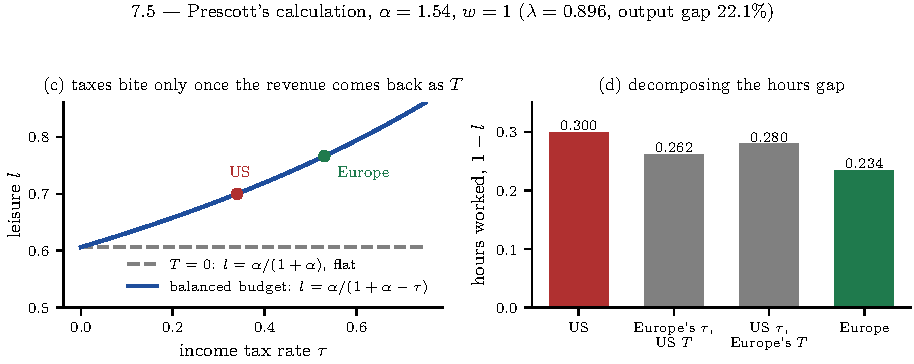
\includegraphics[width=\linewidth]{fig/fig_k7_5_prescott.pdf}\\[3pt]
\captionof{figure}{Problem 7.5. Left: leisure against the tax rate --- flat when revenue is
wasted ($T=0$), rising when it is rebated. Right: the hours gap and the two one-at-a-time
counterfactuals of part (d).}
\label{fig:presc75}
\end{center}

\begin{tcolorbox}[databox]
\texttt{problema\_7\_5} checks the closed form (b) against direct maximisation for both
countries, the $\tau$-independence (c) at five tax rates, the balanced budgets (e) and the
closed form $\alpha/(1+\alpha-\tau)$, the value of $\lambda$ by substituting it back into the
utility equation, and the Frisch elasticity $l/(1-l)$ against a central finite difference of
$1-\alpha c/\omega$ with $c$ held fixed. \checkmark
\end{tcolorbox}
\end{tcolorbox}

%---- Topic: Equilibrium in the Labor Market ----
\subsection{Equilibrium in the Labor Market}

%------- 7.6 -------
% Topic: Equilibrium in the Labor Market
% Keywords: competitive equilibrium, vertical labour supply, Cobb-Douglas, diminishing MPL
\begin{tcolorbox}[evenbox,title={Problem 7.6 \quad The Protestant Work Ethic}]
\begin{tcolorbox}[questionbox]
Suppose that the representative household has preferences given by:
\[u(c,l)=\log(c)+\theta\log(l)\]
where $c$ is consumption, $l$ is leisure and $\theta$ is a parameter. The production function
is given by:
\[F(K,L)=K^{\alpha}L^{1-\alpha}\]
where $K$ is the capital stock, which we take as given and equal to 1, $L$ is labor and
$\alpha$ is a parameter. Firms hire workers in a competitive labor market where the wage is
$w$.\\[3pt]
(a) What will be the equilibrium wage $w$?\\
(b) How does $w$ depend on $\theta$? Suppose the household suddenly develops a so-called
Protestant work ethic and stops enjoying leisure so much, what will happen to real wages?
Explain.
\end{tcolorbox}

\textbf{Solution:}

Following \S7.5, the household is a worker with budget $c=w(1-l)$ (no taxes, no transfers).

\begin{enumerate}
\item \textbf{Labour supply.} First-order condition (7.2.3) with $u'(c)=1/c$ and
$v'(l)=\theta/l$:
\[
\frac{\theta/l}{1/c}=w\;\Longrightarrow\;\theta c=w\,l .
\]
Substitute $c=w(1-l)$:
\[
\theta w(1-l)=w\,l\;\Longrightarrow\;\theta=(1+\theta)\,l\;\Longrightarrow\;
l=\frac{\theta}{1+\theta},\qquad L^s=1-l=\frac{1}{1+\theta}.
\]
The wage cancels: income and substitution effects offset exactly under log utility, so
labour supply is \textbf{vertical} at $1/(1+\theta)$.

\textbf{Labour demand.} The firm maximises $K^{\alpha}L^{1-\alpha}-wL$ (capital given); with
$K=1$,
\[
w=F_L(1,L)=(1-\alpha)L^{-\alpha}.
\]

\textbf{Equilibrium.} Set $L=L^s=\frac{1}{1+\theta}$ in the demand curve:
\[
w=(1-\alpha)\left(\frac{1}{1+\theta}\right)^{-\alpha}
\;\Longrightarrow\;
\boxed{\;w=(1-\alpha)(1+\theta)^{\alpha}\;}.
\]
Output is $Y=L^{1-\alpha}=(1+\theta)^{-(1-\alpha)}$ and consumption is
$c=wL=(1-\alpha)L^{-\alpha}L=(1-\alpha)Y$, the labour share of output.

\item Differentiate:
\[
\dd{w}{\theta}=\alpha(1-\alpha)(1+\theta)^{\alpha-1}>0 .
\]
The wage is \textbf{increasing} in $\theta$. A Protestant work ethic --- enjoying leisure less
--- is a \textbf{fall in $\theta$}, so:
\[
\theta\downarrow\;\Longrightarrow\;L=\frac{1}{1+\theta}\uparrow
\;\Longrightarrow\;w=(1-\alpha)L^{-\alpha}\downarrow,
\qquad Y=L^{1-\alpha}\uparrow .
\]
\textbf{Real wages fall.} The supply curve shifts right along a downward-sloping demand curve.
With capital fixed, each extra hour works with less capital, so the marginal product of
labour --- and the competitive wage --- declines. Output and total labour income
$c=(1-\alpha)Y$ still rise; it is the price of an hour, not the pay packet, that falls.
\end{enumerate}

\begin{tcolorbox}[databox]
With $\alpha=0.35$ and $K=1$ (in the code, \texttt{theta} is the capital share and
\texttt{alpha} the leisure weight):

\begin{center}
\begin{tabular}{@{}ccccc@{}}
\toprule
$\theta$ & $L=1/(1+\theta)$ & $w=(1-\alpha)(1+\theta)^{\alpha}$ & $Y=L^{1-\alpha}$ & $c=wL$\\
\midrule
2.50 & 0.28571 & 1.00771 & 0.44295 & 0.28792\\
1.54 & 0.39370 & 0.90075 & 0.54558 & 0.35463\\
1.00 & 0.50000 & 0.82846 & 0.63728 & 0.41423\\
0.50 & 0.66667 & 0.74911 & 0.76832 & 0.49941\\
\bottomrule
\end{tabular}
\end{center}
E.g.\ for $\theta=1$: $w=0.65\times2^{0.35}=0.65\times1.274561=0.82846$. Going from
$\theta=2.5$ to $\theta=0.5$ raises hours by $133\%$ and lowers the wage by $26\%$. The code
also confirms by direct maximisation that the household's hours are $1/(1+\theta)$ at wages
$0.4$, $1$ and $3$ --- the supply curve really is vertical. \checkmark
\end{tcolorbox}

\begin{center}
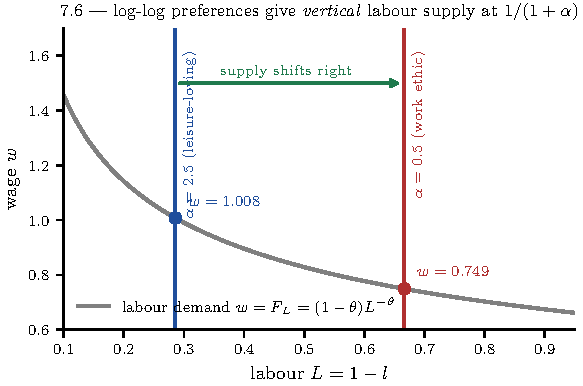
\includegraphics[width=0.72\linewidth]{fig/fig_k7_6_equilibrio.pdf}\\[3pt]
\captionof{figure}{Problem 7.6. Vertical labour supply at $1/(1+\theta)$ against labour demand
$(1-\alpha)L^{-\alpha}$, $\alpha=0.35$. The work ethic moves supply right and the wage down.}
\label{fig:eq76}
\end{center}

\begin{tcolorbox}[trapbox]
The answer assumes the household earns only wages. If it also owns the capital and receives
$\alpha Y$, then $c=Y=wL/(1-\alpha)$, the first-order condition $\theta c=wl$ becomes
$\theta L/(1-\alpha)=1-L$, and
\[
L=\frac{1-\alpha}{1+\theta-\alpha},
\]
which now depends on the wealth effect of capital income --- but it is still decreasing in
$\theta$, so $w=(1-\alpha)L^{-\alpha}$ still falls with a work ethic (for $\theta=0.5$,
$1.54$, $2.5$: $w=0.7937$, $0.9944$, $1.1293$; checked by the code). The sign of the answer
does not depend on who owns the capital; it comes from diminishing returns to labour.
\end{tcolorbox}
\end{tcolorbox}

%------- 7.7 -------
% Topic: Equilibrium in the Labor Market
% Keywords: DMP search model, free entry, matching function, Beveridge curve
\begin{tcolorbox}[oddbox,title={Problem 7.7 \quad The Beveridge Curve}]
\begin{tcolorbox}[questionbox]
Assume the labor market is well described by the search model presented in Section 7.5.\\[3pt]
(a) Suppose there is an improvement in recruiting technology, so that the matching function
becomes $Am(V,U)$, with $A>1$. What happens to the number of vacancies? What happens to the
after-hiring unemployment rate? Would this produce something that looks like a Beveridge
Curve?\\
(b) Suppose there is an increase in the initial (before-hiring) unemployment rate. What
happens to the number of vacancies? What happens to the after-hiring unemployment rate? Would
this produce something that looks like a Beveridge Curve?
\end{tcolorbox}

\textbf{Solution:}

\textbf{A useful rearrangement.} The free-entry condition (7.5.1) with matching function
$Am(V,U)$ reads $\chi=A\,q(V,U)(1-\mu)(y-b)$, with $q=m/V$. Nothing in
$\bar q\equiv\frac{\chi}{(1-\mu)(y-b)}$ depends on $A$, $U$ or $V$, so in equilibrium the
vacancy-filling rate is pinned:
\[
A\,q(V,U)=\frac{A\,m(V,U)}{V}=\bar q
\qquad\Longrightarrow\qquad
\text{matches}=A\,m(V,U)=\bar q\,V .
\]
Substituting into (7.5.2):
\[
\boxed{\;U'=U-\bar q\,V\;}.
\]
After-hiring unemployment is initial unemployment minus $\bar q$ hires per vacancy.

\begin{enumerate}
\item \textbf{Vacancies rise.} At the old $V$, $A>1$ makes $A\,q(V,U)>\bar q$: each vacancy
is filled more often, so posting one now earns more than its cost $\chi$. Firms post more.
Since $q$ is decreasing in $V$ (concavity of $m$), $A\,q(V,U)$ falls as $V$ rises, and entry
stops when it is back at $\bar q$. Formally, differentiating $A\,q(V,U)=\bar q$ at fixed $U$:
\[
q\,dA+A\,q_V\,dV=0\;\Longrightarrow\;\dd{V}{A}=-\frac{q}{A\,q_V}>0\qquad(q_V<0).
\]
\textbf{After-hiring unemployment falls.} With $U$ fixed, $U'=U-\bar q V$ and $V$ has risen,
so $U'$ falls, by $\bar q$ per extra vacancy.

\textbf{Beveridge curve: yes.} Vacancies up, unemployment down --- a negative co-movement. In
fact, with $U$ fixed, every such shock moves the economy \emph{along} the line
$V=(U-U')/\bar q$, with slope $-1/\bar q$ in the $(U',V)$ plane. Shocks to matching efficiency
(and, by the same argument, to anything else that moves $V$ with $U$ given, such as $y$ or
$b$) trace out a downward-sloping Beveridge curve.

\item \textbf{Vacancies rise.} With more job seekers, a vacancy is filled more often: $q$ is
increasing in $U$. At the old $V$, $A\,q>\bar q$, so firms post vacancies until $q$ is back at
$\bar q/A$. Differentiating $q(V,U)=\bar q/A$:
\[
q_V\,dV+q_U\,dU=0\;\Longrightarrow\;\dd{V}{U}=-\frac{q_U}{q_V}>0 .
\]
\textbf{After-hiring unemployment also rises} --- under the standard assumption of a
constant-returns matching function. Then $q(V,U)=m(1,U/V)$ depends only on the ratio $V/U$,
so $q=\bar q/A$ pins $V/U$ at a constant $\kappa$, and
\[
V=\kappa U,\qquad U'=U-\bar q\kappa U=(1-f)\,U,
\qquad f\equiv\frac{Am(V,U)}{U}=\bar q\kappa ,
\]
where $f$ is the job-finding rate, constant and below one. So $U'$ is \emph{proportional} to
$U$: when $U$ rises by 1, $V$ rises by $\kappa$ and $U'$ by $1-f>0$. (Without constant returns
the general expression is $\dd{U'}{U}=1-\frac{m\,m_U}{m-Vm_V}$; constant returns,
$m=Vm_V+Um_U$, reduce it to $1-m/U=1-f$.)

\textbf{Beveridge curve: no.} Vacancies and after-hiring unemployment rise
\emph{together}: a positive co-movement, a ray through the origin in $(U',V)$ space. This does
not trace the curve; it \textbf{shifts} it outward --- each value of $U$ defines its own line
$V=(U-U')/\bar q$, and a higher $U$ is a parallel line further out. In the data, movements
along the curve come from shocks like (a); shifts of the curve, like the outward shift after
2009, point to shocks that change the pool of searchers or the efficiency of matching.
\end{enumerate}

\begin{tcolorbox}[databox]
Kurlat's notation and the code's: $\chi=$ \texttt{kappa}$\,=0.12$, $\mu=$
\texttt{beta\_bar}$\,=0.5$, $y=1$, $b=0.4$, $m(V,U)=0.4\,V^{0.5}U^{0.5}$ (\texttt{A0}$\,=0.4$,
\texttt{gamma}$\,=0.5$); the code's \texttt{hat-U} is $U'$. Then
$\bar q=\frac{0.12}{0.5\times0.6}=0.4$ and the wage is $w=b+\mu(y-b)=0.7$. From
$A\times0.4\,(U/V)^{0.5}=0.4$: $V/U=A^{2}$.

\smallskip
\textbf{(a)} $U=0.08$ fixed; $V=0.08A^{2}$, $U'=0.08-0.4V$, $f=0.4V/0.08$:
\begin{center}
\begin{tabular}{@{}cccc@{}}
\toprule
$A$ & $V$ & $U'$ & $f$\\
\midrule
1.00 & 0.08000 & 0.04800 & 0.40000\\
1.10 & 0.09680 & 0.04128 & 0.48400\\
1.20 & 0.11520 & 0.03392 & 0.57600\\
1.30 & 0.13520 & 0.02592 & 0.67600\\
\bottomrule
\end{tabular}
\end{center}
E.g.\ $A=1.1$: $V=0.08\times1.21=0.0968$, $U'=0.08-0.4\times0.0968=0.08-0.03872=0.04128$.

\smallskip
\textbf{(b)} $A=1$; $V/U=1$, $f=0.4$, $U'=0.6\,U$:
\begin{center}
\begin{tabular}{@{}ccccc@{}}
\toprule
$U$ & $V$ & $U'$ & $V/U$ & $f$\\
\midrule
0.06 & 0.06000 & 0.03600 & 1.000 & 0.40000\\
0.08 & 0.08000 & 0.04800 & 1.000 & 0.40000\\
0.10 & 0.10000 & 0.06000 & 1.000 & 0.40000\\
0.14 & 0.14000 & 0.08400 & 1.000 & 0.40000\\
\bottomrule
\end{tabular}
\end{center}
The code solves (7.5.1) for $V$ with a root finder (no use of $V/U=A^2$) and asserts that $V$
rises and $U'$ falls in (a), that both rise in (b), and that $V/U$ and $U'/U$ are constant in
(b). \checkmark
\end{tcolorbox}

\begin{center}
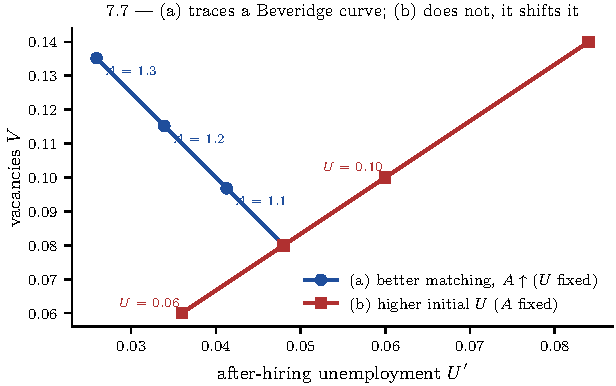
\includegraphics[width=0.76\linewidth]{fig/fig_k7_7_beveridge.pdf}\\[3pt]
\captionof{figure}{Problem 7.7. Experiment (a) moves the economy down a Beveridge curve;
experiment (b) moves it outward along a ray, shifting the curve.}
\label{fig:bev77}
\end{center}
\end{tcolorbox}

%======================================================================
\section*{Companion code}
\addcontentsline{toc}{section}{Companion code}
%======================================================================

Every numerical result above is reproduced by \texttt{Resolucao/kurlat\_ch07\_codigo/}. Each
script checks its analytical formulas against an independent numerical computation and aborts
on any mismatch.

\begin{center}
\begin{tabular}{@{}lp{10.2cm}@{}}
\toprule
\textbf{File} & \textbf{What it does} \\
\midrule
\texttt{ch07\_numerico.py} & Problem 7.1: $l=\theta/w$ against direct maximisation at five
wages, monotonicity of hours, and the log--log contrast. Problem 7.2: both policies solved
numerically, identical $l$, $c$, army and non-army labour. Problem 7.3: the equivalent
$\tau_c$, identical allocation and revenue, three revenue formulas, and the iso-wedge grid.
Problem 7.4: the kinked means-tested budget solved by brute-force grid search against the
segment-by-segment solution, and the non-participation threshold. Problem 7.5: every part,
including $\lambda$, the decomposition and the Frisch elasticity by finite differences.
Problem 7.6: the equilibrium table, the vertical supply, and the capital-income variant.
Problem 7.7: the free-entry condition solved by a root finder for both experiments. \\
\texttt{ch07\_figuras.py} & The four figures. \\
\texttt{estilo\_mpl.py} & \texttt{pgf} backend, so figure text is typeset by \texttt{pdflatex}
with \texttt{lmodern} and \texttt{cmap} and the PDF stays fully copyable. \\
\bottomrule
\end{tabular}
\end{center}

\end{document}
